\documentclass{beamer}


\usepackage{soul}

% TABLES
\newcommand{\ra}[1]{\renewcommand{\arraystretch}{#1}} % spaces in tables
\usepackage{booktabs}   % Allows the use of \toprule, \midrule and \bottomrule in tables for horizontal lines

% LISTS
% \usepackage{enumitem} % Changes the itemize and enumerate


% PSTRICKS
% \usepackage{pstricks,pst-node,pst-tree} % includes graph additions
% \usepackage{pst-pdf} % Compiles the pictures
% \usepackage{pst-node}
% \usepackage{pst-plot}
% \psset{xunit=1cm,yunit=1cm}


% INCLUDE GRAPHICS
\usepackage{graphicx}


% LOGO POSITION
\usepackage{pgf}
% \usepackage[absolute,overlay]{textpos}


% FONTS
% \usefonttheme{serif}
\usefonttheme[onlymath]{serif} % Standard font for math enviroments
\usepackage[T1]{fontenc}
%\usepackage{inconsolata} % Nice monospaced font



% CODE
\usepackage{listings} % Code block (source code) \begin{lstlisting} 

\lstset{
    language=Python,                        % Code langugage
    commentstyle=\color{gray},              % Comments font
    basicstyle=\small\ttfamily,             % Code font, Examples: \footnotesize, \ttfamily
    keywordstyle=\bfseries\color{blue},
    stringstyle=\color{orange},
    numbers=left,                           % Line nums position
    numberstyle=\tiny,                      % Line-numbers fonts
    stepnumber=1,                           % Step between two line-numbers
    numbersep=5pt,                          % How far are line-numbers from code
    numbers=none,
    frame=single,                             % A frame around the code
    tabsize=4,                              % Default tab size
    captionpos=b,                           % Caption-position = bottom
    breaklines=true,                        % Automatic line breaking?
    breakatwhitespace=false,                % Automatic breaks only at whitespace?
    showspaces=false,                       % Dont make spaces visible
    showstringspaces=false,                 % Dont make spaces visible in strings
    showtabs=false,                         % Dont make tabls visible
    belowskip=8pt,
    morekeywords={range, xrange},
    backgroundcolor=\color{white}
    % emph={[2]root,base}
    % morekeywords={one,two,three,four,five,six,seven,eight,
}



\newcommand{\code}[1]{{\small\ttfamily #1}} % \code{inline code}


% BEAMER COLORS
\definecolor{kugreen}{RGB}{50,93,61}
\setbeamercolor{frametitle}{fg=black}
\setbeamercolor{normal text}{fg=black}
\setbeamercolor{structure}{fg=kugreen}

% BEAMER STYLE
\setbeamertemplate{itemize item}{$\bullet$}
\setbeamersize{text margin left=10pt}
\setbeamersize{text margin right=10pt}
\setbeamersize{sidebar width right=0pt}
\setbeamersize{sidebar width left=0pt}
\setbeamercolor{block title}{fg=white,bg=kugreen}
\setbeamercolor{block body}{fg=black,bg=white!95!black}


% BEAMER HEADLINE
\setbeamertemplate{headline}
{%
    % \vbox{

    % \vspace{2pt}

    % \hspace{10pt}
    % \tiny
    % \rmfamily
    % \expandafter\insertshortauthor
    %     \vspace{1pt}
    % }
}


% BEAMER TITLE
\setbeamertemplate{frametitle}
{
    \color{kugreen}
    \begin{centering}\medskip
        \insertframetitle\par
    \end{centering}
}


% BEAMER FOOTER
\setbeamertemplate{footline}[text line]
{%
    \vbox{%
        \tiny\ttfamily
        \insertvrule{0.5pt}{kugreen}

        \vspace{2pt}

        \strut{
        \rmfamily\itshape
        \expandafter\insertshorttitle
        \expandafter\insertauthor,
        \insertshortinstitute
        }
        \hfill\strut{
        }
        \hfill\strut{
            \insertframenumber\,/\,\inserttotalframenumber
            % 
\includegraphics[width=20pt,natwidth=610,natheight=642]{KUNATLogo.pdf}
        }

        \vspace{1pt}
    }
}

\setbeamertemplate{background}{
    % \hspace{330pt}
\includegraphics[width=25pt,natwidth=610,natheight=642]{KUNATLogo.pdf}
}

% BEAMER Frontpage
\setbeamertemplate{title page}
{

    \begin{beamercolorbox}[center]{beamer color}

        {
            \huge
            \color{kugreen}
            \inserttitle
        }
        \bigskip
        \bigskip

        
\includegraphics[width=2cm]{KUNATLogo}

        \bigskip
        {
            \bf
            \rmfamily
            {\large \insertauthor}
        }

        \smallskip
        {
            \rmfamily
            \footnotesize
            \insertinstitute
        }

        {
            \rmfamily
            \footnotesize
            \insertdate
        }

    \end{beamercolorbox}


    \addtocounter{framenumber}{-1}
}

% Removes the navigation bar
\beamertemplatenavigationsymbolsempty

% CONTENT

\logo{\pgfputat{\pgfxy(-1,-0.435)}{\pgfbox[center,base]{
\includegraphics[width=1.2cm,natwidth=610,natheight=642]{KUNATLogo.pdf}}}}



\title[]{Molecular Statistics, Week "5"}
\institute[University of Copenhagen]{Department of Chemistry \\ University of Copenhagen}
\author[Jimmy Charnley Kromann]{Jimmy Charnley Kromann}
\date{2014}

\begin{document}

\frame[plain]{\titlepage}


\begin{frame}[fragile]

    \frametitle{Week "5", Overview}

    todo for this week; useful tips for your bachelor/future science

    \begin{itemize}
        \item More plotting
        \item Data analysis
        \item print format
        \item Monte Carlo pi
        \item Debug
    \end{itemize}

\end{frame}


\begin{frame}[fragile]

    \frametitle{Plotting stuff example}

    \begin{align*}
        \Delta G^\circ = \Delta U - T \Delta S^\circ + \Delta W + \delta
    \end{align*}

    \begin{columns}[t]

        \column{0.4\linewidth}

            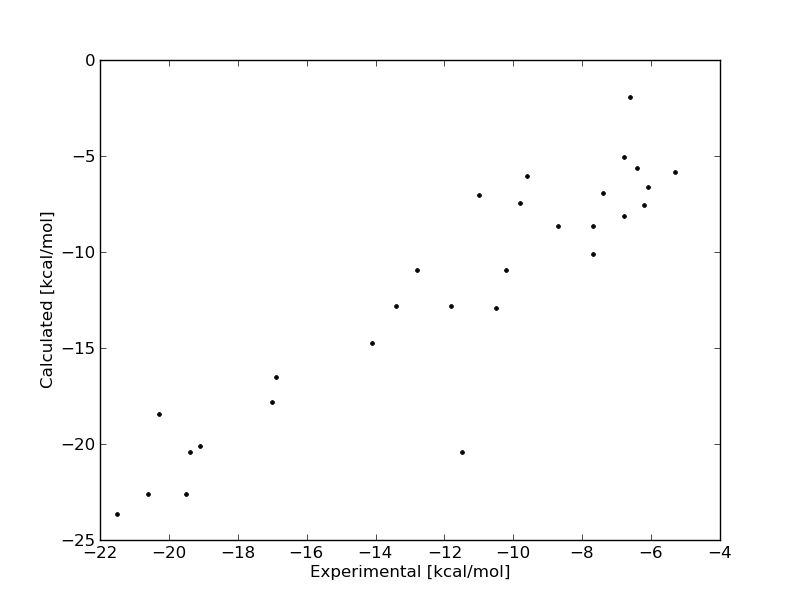
\includegraphics[width=1.2\textwidth]{images/binding_energy.png}

        \column{0.4\linewidth}

            2x files

            The columns:\newline ID, $\Delta U$, $\Delta W$, $\Delta S^\circ$

            $\delta = -5.83$, $T = 298.0$

    \end{columns}

\end{frame}


\begin{frame}[fragile]

    Data analysis

    \begin{itemize}
        \item Calculate the Root-mean-square deviation (RMSD)

        \begin{align*}
            \mathrm{RMSD} = \sqrt{\frac{\sum_i^N (x_{\mathrm{exp},i}-x_{\mathrm{cal},i})^2 }{n}}
        \end{align*}

    \end{itemize}

    \begin{itemize}
        \item Calculate the Pearson Correlation factor r and corresponding p value.
    \end{itemize}

    Hint: search for the scipy module for a nice Pearson function

\end{frame}


\begin{frame}[fragile]
    Print format

\begin{lstlisting}
print "{0:5d}".format(42)
\end{lstlisting}

\begin{lstlisting}
"{0:5d}".format(42) # integer
"{0:5.2f}".format(65.6789) # float
"{0:5s}".format("hello") # string
\end{lstlisting}

https://docs.python.org/3/library/string.html\#formatspec

\begin{lstlisting}
print "{0:5d} & {1:5.2f} & {2:5.2f} \\\\".format(i, list_Ge[i], list_G[i])
\end{lstlisting}


\end{frame}


\begin{frame}[fragile]

    % http://www.eveandersson.com/pi/monte-carlo-circle
    % How this program works:
    %
    % If a circle of radius R is inscribed inside a square with side length 2R,
    % then the area of the circle will be pi*R^2 and the area of the square
    % will be (2R)^2.
    % So the ratio of the area of the circle to the area of the square will be
    % pi/4.
    %
    % This means that, if you pick N points at random inside the square,
    % approximately N*pi/4 of those points should fall inside the circle.
    %
    % This program picks points at random inside the square.
    % It then checks to see if the point is inside the circle (it knows it's
    % inside the circle if x^2 + y^2 < R^2, where x and y are the coordinates
    % of the point and R is the radius of the circle).
    % The program keeps track of how many points it's picked so far (N) and how
    % many of those points fell inside the circle (M).
    %
    % Pi is then approximated as follows:
    %
    %           4*M
    %      pi = ---
    %            N
    %
    % Although the Monte Carlo Method is often useful for solving
    % problems in physics and mathematics which cannot be solved by
    % analytical means, it is a rather slow method of calculating
    % pi.
    % To calculate each significant digit there will have to be
    % about 10 times as many trials as to calculate the preceding
    % significant digit.

    Monte Carlo simulation

    \begin{align*}
        % A_\text{circle} &= \pi \cdot r^2 \\
        % A_\text{square} &= 4 \\
        % r &= 1 \\
        \pi &= 4 \cdot A_\text{circle} / A_\text{square}
    \end{align*}

    \begin{equation*}
        x^2 + y^2 < r^2
    \end{equation*}

    \begin{itemize}
        \item Calculate Pi (using Monte Carlo)
        \item How many steps before converge?
    \end{itemize}

\end{frame}


\begin{frame}[fragile]

    More Debug


\end{frame}


%%%%%%%%%%%%%%%%%%%%%%%%%%%%%%%%%%%%%%%%%%%%%%%%%%%%%%%%%%%%%%%%%%%%%%
%% END FRAMES
%%%%%%%%%%%%%%%%%%%%%%%%%%%%%%%%%%%%%%%%%%%%%%%%%%%%%%%%%%%%%%%%%%%%%%

\end{document}

